% !TEX root = ../../report.tex

\section{State Of The Art}

The following section will present the state of the art recommender systems...

\subsection{System Coldstart Handling}

%When does the system go from a cold->warm?
%When can a user be considered warm? (How many ratings?)
%When can a item be considered warm? (How many ratings?)

In the literature, the term cold is used about an object in a system, or a whole system, which is new. Cold-start scenarios in recommender systems are situations in which little/no prior events, like ratings or clicks, are known for certain users or items. The cold-start problem can therefore be divided into three sub problems:

\begin{itemize}
	\item \emph{Cold-start system}: A situation where we only have new users and little or no ratings for the items.
	\item \emph{Cold-start item}: The problem of recommending items that are new to the system, which have not received any ratings. E.g. in a scenario where the average item in an item collection have 10 000 ratings, a new item with only 5 ratings would be considered an "cold-item"
	\item \emph{Cold-start user}: The problem of giving accurate recommendations who is new to a recommender system. E.g. in a recommender system where the average user have rated 100 items, a user which only have rated 2 items, would be considered a "cold-user".
\end{itemize}

The cold-start system problem is mainly a collaborative filtering problem, and can be seen as a combination of the cold-start user and cold-start item problem where the majority of the users are new to the system and have expressed few preferences, resulting in a very sparse user-item matrix, rendering recommendation systems using traditional collaborative-filtering methods futile.

The cold-start user problem is present both in content-based and collaborative-filtering systems. In content-based systems, the lack of ratings given by the target user, means that the target user will have a limited content-profile, since the users content profile is constructed using content-information from his/hers rated items. Similarly, the cold-start user problem also affects user-based collaborative filtering, since user similarities are calculated based on items that a user shares with other users of the system. The system will therefore most likely struggle to find users with tastes that are \emph{truly} similar to the target user. In both cases, recommendation quality is most likely bound to suffer.

%TODO  Cite articles using content-information to tackle the cold start item problem
The cold-start item problem. In content-based systems, new items can easily be recommended using the content information of the item, making it a popular solution \cite{} to the cold-start new item problem. This problem is more severe in collaborative-filtering systems where items are only recommendable if they have been rated by multiple users. New items will therefore not be recommendable before multiple users somehow stumble upon the new item while e.g. browsing the item collection, unless additional measures are taken to solve this problem.

%Other snippets worth including
%#1
However in a typical domain, for example in the domain of movies or books, the number of items is very large (in the order of the millions) while the number of items rated by every single user is in general small (in the order of dozens or less). This means that it is very unlikely two random users have rated any items in common and hence they are not comparable.

%#2
One crucial problem of recommender system is how to best learn from new users. Collaborative Filtering (CF), is the best known technology for recommender systems and is based on the idea that like-minded users have similar tastes and preferences. A new user therefore poses a challenge to CF recommender, since the system has no knowledge about the preferences of the new user, and can therefore not provide any personalized recommendations, this is known as the cold start problem for new users. The system must therefore acquire some information about the new user in order to make personalized recommendations.

\subsubsection{Cold-start system}

In this section we will present a few different solutions to the cold-start system problem found in the literature. As mentioned in the introduction to the cold-start problem, most algorithms only work effectively in environments where the dataset has high information density. In fact, in extreme cases, when data is very scarce, simple non-personalized recommendations based on global averages can outperform collaborative-filtering and content-based algorithms. Pure collaborative filtering cannot help in a cold-start setting, since no user preference information is available to form any basis for recommendations.

%Propose a categorization of approaches
	%Initial Categorization
		%The immediate remedy - Meta information (Hybrid approaches)
		%Blending/Non personalized approaches/Global models for all users
		%Seed items or users
			%Wisdom of the Better Few: Cold Start Recommendation via Representative based Rating Elicitation
		%Trust-Aware Collaborative Filtering
			%Trust-Aware Collaborative Filtering for Recommender Systems
			%+ many others
		%Filterbots / surrogate users
			%Na¨ıve Filterbots for Robust Cold-Start Recommendations
				%Check out RipperBots (For binary rating version)
				%Recommend items based on the average of the users with the same demographics...

%Read a few articles that fall under each category and present them
%Discussion: Which are the most relevant?
	%How do we determine what is the best solution?

\paragraph{Trust Aware Recommender Systems}

%General Introduction
%	Explain the main idea behind TRUST AWARE RECOMMENDERS formally + figures
%	See - Trust-Aware Collaborative Filtering for Recommender Systems for formal description

Due to the popularity of social networks such as Facebook, more and more researchers turn to incorporate the social relationships (e.g. trust) of users to help complement users’ preference in addition to item ratings. Trust relationships of users are often employed in order to correlate more potential raters for the active users who require recommendations.

% Web of Trust - Figure explanation
Using explicit trust statements, it is possible to predict trust in unknown users by propagating trust. Consider the example shown in Figure \ref{figure:weboftrust}. User A has issued a trust statement in B and C; hence B and C are in the web of trust of A. Using these explicit trust statements, it is possible to predict trust in unknown users by propagating trust, making it possible to infer something about how much user A could trust D.

\begin{figure}[H]
    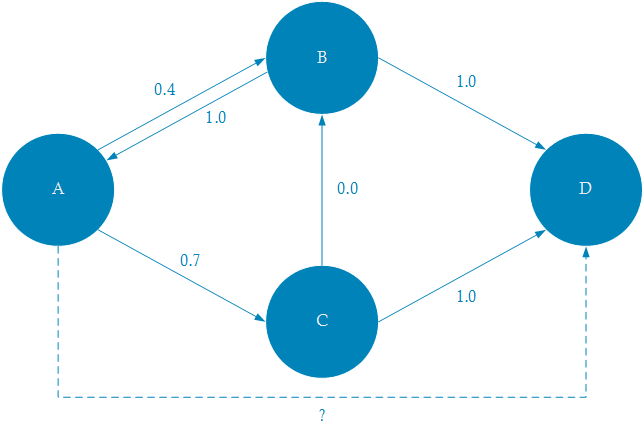
\includegraphics[width=5in]{image/webofTrust.png}
    \centering
    \caption[Trust Network]{Trust Network. Nodes are users and solid edges are trust statements. The dotted edge is one of the undefined and predictable trust statements (Adopted from \cite{Massa2004}}
    \label{figure:weboftrust}
\end{figure}

% The formals
To capture all the trust statements we need a $NxN$ matrix, where $N$ is the number of users, since each user is allowed to express a trust value in every other user. This matrix will make up our trust network among the users. If $u$ trusts $v$, then there is a value $t_{u,v}$ for this trust which is a real number in $[0,1]$. Zero means no trust and one means full trust. In addition to the trust network we will also have a Rating matrix of size $NxM$, where $M$ is the number of items. This rating will not differ from a standard rating matrix, which are used in traditional collaborative filtering systems. The value $r_{u, i}$, is the rating user $u$ have given to item $i$, the rating scale may differ from system to system.

% Architecture 
The systems takes as input the trust network (representing the trust statements) and the ratings matrix (ratings given by users to items) and produces, as output, a matrix of predicted ratings that the users would assign to the items. Figure \ref{figure:trustarchictecture} shown a conceptual overview of the trust-aware recommender system architecture.

\begin{figure}[H]
    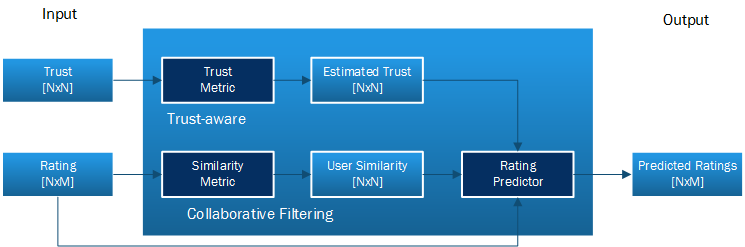
\includegraphics[width=5in]{image/trustawarearchitecture.png}
    \centering
    \caption[Trust-Aware Recommender System Architecture]{Trust-Aware Recommender System Architecture. Adopted from \cite{Massa2004}}
    \label{figure:trustarchictecture}
\end{figure}

The \emph{Trust Metric} module takes the trust network as input, and exploits trust propagation in order to predict, for every user, how much she could trust other users. Trust metrics can either be local and global. Global trust metrics produces an estimated trust matrix with all the rows equal, meaning that the estimated trust in a certain user (column) is the same for every user (row). A simple local trust metric could e.g. for each user assign to every other user a predicted trust based on her minimum distance from the source user. More sophisticated ones could also be employed. If we again consider Figure \ref{figure:weboftrust}, we could employ a local trust metric where the predicted trust is based on the minimum distance from the source user. If we set the maximum propagation distance $d$, a user at distance $n$ from the source user will have a predicted trust value of:

\begin{equation}
t_{u,v} = (d-n+1)/d
\end{equation}

Giving users not reachable within the maximum propagation distance a trust of $0$. Using user $A$ as the source user, the users at distance $1$ ($B$ and $C$) would get a trust value of $(4-1+1)/4 = 1$, while the user at distance 2 (D) would get a predicted trust value of $(4-2+1)/4 = 0.75$. Meaning that we will have a linear decay in trust based on the distance from the source user.

The \emph{Similarity Metric} module computes the user similarities, this is one of the standard steps of any traditional collaborative filtering technique, user similarities can be found e.g. by using the Pearson Correlation Coefficient. The intuition is that, if a user rates in a similar way to another user, then her ratings are using for predicting the ratings for that users. 

The \emph{Rating Predictor} can use the neighbours from the user similarity matrix, the estimated trust matrix or a combination of both in order to calculate the predicted ratings.

The main advantage is not improved accuracy, but improved coverage. As exemplified by Massa et. al. \cite{Massa2007}. The authors attempted propagating the trust up to a distance of 4. By using the Pearson Correlation coefficient they found on average 160.73 neighbours. However just propagating a few steps help to increase significantly the number of neighbours that can be considered for rating predictions. Propagating at distance 2 (friends of friends) it is possible to reach 399.89 users, further increasing the trust horizon to 3 and 4 allows respectively 4,386.32 and 16,333.94 users. This pattern is even more evident on cold start users \cite{Massa2004}. These results say that by propagating trust it is possible to increase the coverage (generate more recommendations) but that it also considers users who are worse predictors for the current user so that the prediction error increases as well. The trust propagation horizon basically represents a trade-off between accuracy and coverage.

% Trust-Aware Collaborative Filtering for Recommender Systems
%	Main improvements - Users with few ratings
% 	Requires user involvement - Allows user to rate other users
%	Findings:
%		Little improvement in accuracy
%		Much better coverage
%			For users with 4 ratings:

% You might think:
% 	"What about the scalability issues of having 3-4 times as many connections?"
% 	Solution: Only consider a "few" selected users based on their "predicted trust" (cutoff point)


% Trust-aware Recommender Systems
% Article Comments:
% 	Requires user involvement - is this a acceptable?

Massa et. al. \cite{Massa2004, Massa2007} propose using trust information explicitly expressed by the users. Users are allowed to state how much they consider every other user trustworthy that, in the context of recommender systems, is related to how much they consider the ratings provided by a certain user valuable and relevant. This additional information (trust statements) can be organized in a trust network and a trust metric can be used to predict the trustworthiness of other users as well (for example, friends of friends). The idea here is to not search for similar users as CF does but to search for trust-able users by exploiting trust propagation over the trust network. The items appreciated by these users are then recommended to the active user. In decentralized environments where everyone is free to create content and there is no centralized quality control entity, evaluating the quality of the content becomes an important issue. This phenomenon can be observed in online marketplaces such as E-bay where users can create "fake" auctions, peer-to-peer networks where peers can enter corrupted items. In these environments, it is often a good strategy to delegate the quality assessment task to users themselves.

The authors experimented with both Local Trust Metrics and Global Trust Metrics. They used the PageRank algorithm as a global trust metric. PageRank tries to infer the authority of every single user by examining the structure of the network. The algorithm follows a simple idea: if a link from user A to user B represent a positive vote casted by A to B, then the global rank of a page depends on the number (and quality) of the incoming links. The trust values assigned by users to users are used to predict the trustworthiness of unknown users. Their findings, not surprisingly, indicate that Global Trust Metrics are not suited for the task of finding good neighbors, especially for providing personalized recommendations. As a local trust metric they chose MoleTrust, which is a depth-first graph walking algorithm with a tuneable trust horizon which allowed them to experiment with different propagation distances.

%Motivation / Rational for their approach






%Alleviating the Sparsity Problem of Collaborative Filtering Using Trust Inferences
%Article Comments:
%	- Pretty good general model for dealing with sparsity
%	- Requires no additional information such as product details, demographic information about userstrus

Papagelis et. al. \cite{Papagelis2005} proposed to alleviate sparsity using trust interfaces. Trust interfaces are transitive associations between users in the context of an underlying social network. Their approach is built on the idea of social networks in recommender systems. Instead of reducing the dimension of the user-item matrix, in an attempt to make it more informative, they propose a method that permits to define transitive properties between users in the context of a social network.

\begin{figure}[H]
    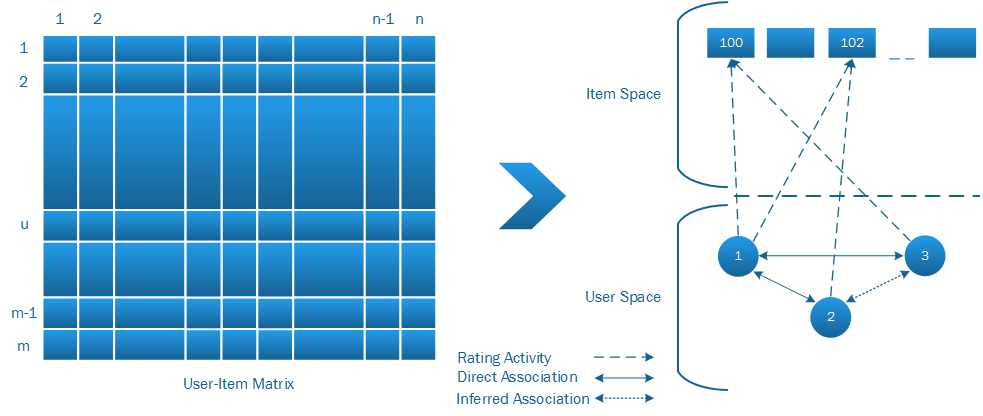
\includegraphics[width=5in]{image/trustnetwork.png}
    \centering
    \caption[Underlying Social Networks in Recommender Systems]{Underlying Social Networks in Recommender Systems}
    \label{figure:cfsocialnetwork}
\end{figure}

Due to the number of ratings that exist in recommendation systems, underlying social networks are very sparse. There are cases in which insufficient or loss of information is detrimental for the recommendation algorithms. Consider Figure \ref{figure:cfsocialnetwork}, classic CF will associate only the users which have co-rated an item (User $1$ and $2$ and user $1$ and $3$). To deal with the problem of a sparse social network, it is possible to infer trust between a source user $S$ and a target user $T$ through an intermediate user $N$ (User $2$ and $3$ are connected through the intermediary user $1$), as shown by the \emph{Inferred Association} arrow. According to this process, trust is propagated in the network and associations between users are built, even if they have no co-rated item. Trust paths can be of variable length, depending on the number of associations that one needs to traverse in order to reach the target user.




% Using a Trust Network to Improve Top-N Recommendation
% Article Comments:
%		-

Jamali et. al. \cite{Jamali2009} propose two different methods for getting around the cold-start user problem using a trust network.

Approach 1: Random Walk
Starting from user $u$, we perform a random walk on the trust network. Each random walk stops at a certain user. Then the items rated highly by that user will be considered as recommended items, ordered according to the ratings expressed by that user. We perform several random walks to gather more infroamtion and compute a more confident result. The estimated rating of each item is the average of ratings for that item over all raters considered. At the end, we output items with the highest estimated rating as top-N recommended items.

Approach 2: Combined Approach
In this approach we compute the top $K$ trusted users in the network and rank the items rated by these trusted users to compute top-N recommended items. We use the collaborative filtering approach to compute another set of top-N recommended items. Finally, we merge these two lists to produce a combined list of top-N recommended items. The top $K$ trusted users can either be found by \emph{Breadth First Search} or \emph{Random Walk in the social network}.

%Random walk with depth = 2, best result, however, it does not outperform CF-User...

\paragraph{Hybrid Methods}

The cold start problem, is in its most basic form, a consequence of lacking data or information. Hybrid methods incorporate information from other sources the bridge the gaps, and improve the recommendation quality.

\subsubsection{Cold-start user}

%Introduction
%Cold start users often account for more than 50% of the total users

The difficulty in the new user problem is how to find the neighbours of a new user effectively.

This section will present a few different solutions to the cold-start user problem proposed in the literature

%Can the different approaches be classified? E.g. 3 main categories of approaches
	%Initial categorization
		%Interview process to quickly learn user preference/Ask to rate, Intelligent selection
			%Information theory vs most popular, How do one select the items to present to the user?
				%Rashid2002, Rashid2008
 			%Decision trees
 				%Functional Matrix Factorizations for Cold-Start Recommendation
 		%Hybrid approaches
 			%Using demographic data - KEEP IN MIND: What kind of demographic information is most commonly used? / Most informative in our case?
 		%Key figures / Seed users. TODO : For later, check with Seed items or users (Cold-start system)
 			%Whom Should I Trust? The Impact of Key Figures on Cold Start Recommendations
 		%Trust-aware / Trust propagation

%Read a few articles from each category
%Discussion: Which category/approach is the most relevant for us?
	%How do we determine this "systematically"?

\paragraph{Intelligent Selection}\mbox{}\\

%My though behind including these articles:
%Use e.g. a tinder like interface and ask the user to like/dislike 15 items when first logging in

\begin{chapquote}[30pt]{Vanessa Redgrave}
  "Ask the right questions if you're going to find the right answers"
\end{chapquote}

As pointed out by Rashid et. al. \cite{Rashid2002}, the most direct way of acquiring information for use in personalised recommendations from a new users is to present item for the user to rate. However, they argue that the system must be careful to present useful items to garner information. A food recommender should probably not ask whether a new user likes vanilla ice cream since most people like vanilla ice cream. Therefore, knowing that a new user likes vanilla ice cream tells you very little about the user. The choice of what questions to ask a new user, then, is critical. The authors performed a study of different item selection strategies that collaborative filtering recommender systems can use to learn about new users. They presented the users with a questionnaire with items asking them to rate/select the ones they like. Their strategies can be divided into five classes:

\begin{itemize}
\item \emph{Random:} strategies: Strategies that avoid bias in the presentation of bias
\item \emph{Popularity:} Select among the top N items where the probability that an item is selected is proportionate to the items popularity.
\item \emph{Pure entropy:} Present the items with the highest entropy that the user has not seen
\item \emph{Balanced strategies:} A balanced approach combining both popularity data and entropy.
\item \emph{Personalized:} As soon as some information is known about a user, present items specifically tailored to that user using e.g. item-item similarity
\end{itemize}

Their evaluation focused on user effort and accuracy. Their suggestion for e-commerce recommender system is to start off recommending the most popular items rather than the highest rated ones, and then use item-item similarity as quickly as possible.

This study was later extended by Rashid et. al. \cite{Rashid2008} where they more closely examined information theoretic strategies for item selection. In the article they identify a number of aspects that a new user preference elicitation strategy should consider.

In the article they introduced three new strategies:

\begin{itemize}
\item \emph{Entropy0}: Entropy Considering Missing Values
\item \emph{HELF:} Harmonic mean of Entropy and Logarithm of Frequency
\item \emph{IGCN:} Information Gain through Clustered Neighbors
\end{itemize}

%TODO Sum up the approaches, neatly

%Findings:
%#1 IGCN
%#2 Entropy0
%#3 HELF
%#4 Popularity

%Discussion on "suitedness", user involvement ∕ recommendation quality tradeoff
It is worth mentioning that the authors worked on the cold-start new user problem for a movie recommender. The implications of this is that a user must have watched a movie, in order to rate it. This is not so important for our domain, as taking a quick look at the item should be sufficient to like/dislike it.
%Implications -> Ignore the user effort stars in the article, as they dont have to browse until they find movies they previously have watched
%Priority: Making the tinder like "swipe" interface smooth and efficient is important, making the rating as easy as possible
%We cannot calculate entropt as we have no rating distribution for the items (1-5), damn u implicit feedback ;)

We are constrained to unobtrusively learn user-profiles from the natural interactions of users with the system, meaning that we can not require the user to rate e.g. 10 items before we can start providing recommendations. We currently have a \emph{mixed initiative} system meaning that there is provisions for both user and system controlled interactions. We (the system) can only select which items to recommend to the user, and this does not mean that the user actually will click an item or rate it.

\paragraph{Hybrid Approaches}

It is a common strategy to gather demographic data in order to gain knowledge about the user. Data that may be collected typically includes age, gender, nationality, marital status, income, educational level and occupation. The idea is that people with a more common background share a more similar taste than someone with a random background, and therefore good recommendations can be made as long as we know the new user’s background.



\subsubsection{Cold-start item}

To solve the new-item problem, there are two commonly used (simple) solutions that often are used in E-commerce websites:

\begin{itemize}
\item Advertising at the homepage/front-page of the website, putting the new items in an eye catching position. This solution, however, may 		result in that some users, which don't like these new items, might leave the website.
\item Requesting the user to choose one or more of his/hers categories while registering for the site, and recommend items from the selected categories. This approach however, requires active user involvement and complicates the sign up process -> BAD, in addition, many users might chose not to give up any personal interest information, thus the user group covered by this solution is not large enough.
\end{itemize}

This section will cover some approaches described in the literature to solve the cold-start new item problem.

%What strategies exist? Categorization
	%Most dominant! Hybrid approach incorporating item information
	%Dynamic Browsing tree
		%Collaborative Filtering Cold-Start Recommendation Based on Dynamic Browsing Tree Model in E-commerce


\paragraph{Hybrid Methods / Latent Factor Models}

%TODO - Sort articles, some are more general cold-start solutions (not just new-item)
%TODO - Read articles more in detail, explain their approaches

%Regression-based Latent Factor Models

Agarwal et. al. \cite{Agarwal2009} propose a class of latent factors models called RLFM that incorporates both user/item features and past interaction data into a single model.

%Learning Attribute-to-Feature Mappings for Cold-Start Recommendations
% - Model for positive implicit feedback!
% - Demonstrates usefulness for new-item recommendations


%fLDA: Matrix Factorization through Latent Dirichlet Allocation
% -
Matrix factorization method to predict ratings in recommender system applications where a "bag-of-words" representation of item meta-data is natural

%Matchbox: Large Scale Bayesian Recommendations
% - Online algorithm
The Matchbox system makes use of content information in the form of user and item meta data in combination with collaborative filtering information from previous user behavior in order to predict the value of an item for a user.

%What is suitable in our case?/Discussion
%TODO

\subsection{Fashion Recommendation}

\subsubsection{Psychology something}

% -----------------------Article notes START------------------------------

% Fashion article notes (yeah will move to github-page):
% fashion marketing and theory:

% Difference between men and women - what, where, when and how
% Understanding of consumer behavior can come from different ares, such as: psychological, cultural social psychological, physio-psychological, genetics anthropology.
% Fashion is a socio-cultural phenomenom.
% New fashion starts with the refusal of what is olad
% Some question fashion must answer:
%     - Handling different seasons
%     - market segment
%     - product amount
%     - price
%     - consumer needs and prefs
%     - channels to distribute product
%     - organize and control sales
% Thought: Must recommend based on what is fashion, make fashion.
% Companies must:
%     - find consumer needs
%     - consumer segment, how to approach
%     - pos to reach segment
%     - reqs of the segment
%     - price
%     - channel distr demands
%     - sails strats at segment
% buying behavior:
% societal communication factors grant and spephen
% main factors:
%     - phsiological factors
%     - socio-cultral factors
%         family - strong on younger ppl
%         firends
%         work
%         focial groups
%     - personal factors
%         age
%         life cycle
%         occupation
%         economical level
%         way of life
%         personality
%     - psychological factors
%         more expensive because more expensive - increase self-confidence
%     - rational factors
% garment evaluation
%     - concrete
%     - attributes
%     - abstract
%     - intrinsic
%     - extrinsic
%     - aesthetucs
%     - price
%     - brand
%     - fun
%     - style
%     - color
%     - country of origin
%     - entertainment
%     - pattern
%     - fabric
%     - salespersons eval
%     - enjoyment
%     - aooearence
%     - approval of others
%     - need
%     - fashionability
%     - cooridnation with wardrobe
%     - function
%     - utiliatian
%     - duarvaility
%     - comfoirt
%     - quality
%     - fit
%     - care
% modern consumer: pleasure with consumption exp itself
% The stages of the consumer:
% 	the need
% 		internal stimuli:
% 			thirst
% 			hunger
% 			tired
% 			personal interests
% 			motivation (checkout motivation theory... Kotler and Keller, 2005; McEnally and Chernatony, 1999, De Brouwer 2009, Guillen-Royo, 2008) allows understaning the first stage, the acknowledgement of a need)
% 		external stimuli:
% 			commercial
% 			other persons
% 	information search
% 	making the evaluation of alternatives
% 	purchase decision
% Consumer buying behavior:
% 	Process of consumer use to select, secure, use and dispose of products
% interesting: We potentially miss those beliefs and attitudes held at the unconscious or implicit levei that can be crucial to determining consumer behaviour. Also the memory that people hold on their consumer experiences will drive both aversion and preference towards products. Aversion behaviour is our avoidance of certain things (brands or marketing offers) made to us as consumers.
% 	The impilicit memory registers vast amounts. Consumers often make brand choices intuitive, and cannot tell why they mad that choice.
% 	Behavior is predominantly determined by intention
% 		attitude
% 		subjective norms
% 		precieved bahavior control
% 	The ecpectation.confirmation model. (oliver 1980)
% 		post purchase behavior.
% 		repeat purchase
% 		if percieved performance mettes expectation, confirmation is formed and consumeris satisfied.... no shit
% 			satisfied consumers are more likely to purchase the same prodct again - map this to stores? to view amount? i.e. revisit an item -> item satisfaction -> want (yes, but science?)
% otts (1989)
% 	culture is one of the main factors to determine behavior - culture from facebook = userbehavior
% 	external:
% 		culture
% 			culture
% 			cubculture
% 				nationality
% 				religious
% 				racial
% 				geographical
% 			social class
% 		physical environment
% 	internal:
% 		physological
% 		psycholocial factors
% 			human desire
% 	everyone is included in subcultures - find these sub cultures. pink(color)
% 	forming subgroups
% 		find someone who mathes yourself and make smaller group together
% 	individual lifestyle
% 		personality
% 		exteranal factors
% 			culture
% 			daily facotrs
% social psychology (albanese 1989)
% 	understanding behavior in presence of other individuals of groups
% 	social perceptions
% 	social influencechr
% 	social rewards
% 	peer pressure
% 	social cues
% 	social sanctions
% physiopyscholoical
% 	study of the interaction of the boy with the mind
% 	bbehavior is caused by physical and chemical phenomena in the bods morris 1996
% 	hypothalamus - control consumption - hunger = reduced consumer constraint? = higher purchase before eatingtimes? find eatingpattern :P
% genes direct our consumption behavior
% 	programmed to work consume in a special way - how to use it
% Business anthropology
% 	become the hotest candidates for busness related resarch hobschr

% -----------------------Article notes END------------------------------

% -----------------------Article notes START------------------------------
The Psychology and Behavior of Consumers in the
Fashion Industry

% -----------------------Article notes END------------------------------

% n:
% http://ieeexplore.ieee.org/xpl/login.jsp?tp=&arnumber=5581949&url=http%3A%2F%2Fieeexplore.ieee.org%2Fxpls%2Fabs_all.jsp%3Farnumber%3D5581949
% http://link.springer.com/chapter/10.1007%2F978-3-540-79355-7_8
% http://link.springer.com/chapter/10.1007%2F978-3-540-79355-7_8
% http://onlinelibrary.wiley.com/doi/10.1002/ecj.10261/pdf
% http://www.slideshare.net/guest2f8cee8/polyvore-outfit-recommender-system
% http://link.springer.com/chapter/10.1007/978-3-540-72559-6_18
% http://link.springer.com/article/10.1007/s10458-007-9021-x
% http://dl.acm.org/citation.cfm?id=1216368
% http://dl.acm.org/citation.cfm?id=245124
% http://link.springer.com/chapter/10.1007/11833529_64
% http://dl.acm.org/citation.cfm?id=1345466
% http://www.sciencedirect.com/science/article/pii/S0957417402000520
% http://link.springer.com/chapter/10.1007/978-3-540-72079-9_10


\subsubsection{Fashion Recommender}

SuitUp:
Social network which attempts to be a "practcal and ejoyable social space centered around clothing items".
Use multiple tools for recommending colts, including a Hot-or-Not, following other users, rate items and outfit creator approach.
Developed based on users surveys, brainstorming sessions and interviews with potential users.
The potential users consisted of a group of about 70 people who where in their 20's.
Hard to keep up with the changing in fashion and the users preferences.
Generates clothing and neighbor recommendations for users.
DirectedEdge~\cite{direcetedEdge} is used for recommendations.
It treats everything as an item, whether it is a user or a piece of clothing.
This makes item-item, user-user and item-user correlations simple.

SuitUp Finding:
The Hot-or-Not approach was well liked by all the test subjects.
Some more, but not very relevant.
sauce:\cite{SuitUp}

LookBook:
Can stay on the "new"/"hot" page for about 1-2 days.
This happens with up voting from other users.
So in other terms, something says popular for 1-2 days...

DirectedEdge:
Recommendation API.
Can handle easily the need to express more interest in new items.
Which makes it useful in a fashion domain where items has a short lifetime.
%http://developer.directededge.com/
Twitter example:
Obama is just noise when it comes to suggesting new friends to follow.
The authorative source is noise.
Tell me something i don't know problem.


% Building Recommender Systems using a Knowledge Base of product semantics
% http://images.accenture.ca/SiteCollectionDocuments/PDF/recommenderws02.pdf
% 	- Would probably require some more product semantics...

%What are the challanges of making recommendations for fashion?

%	- For how long are items relevant?
	%	- Spring, Summer, Fall, Winter collections
			%Improving E-Commerce Recommender Systems by the Identification of Seasonal Products (Article)
	%	- Freshness, fresh decay operators

%	- Implicit feedback (Based around users fashion browsing habits and an occational purchase...)
	%	- What do we look at? What information is the most useful
	%		- Item category, item keywords, brand... ?

%	- Changing interest of users
%	- Unstructured content/multiple content providers
	% - How to select features for a content-based approach
		% E.g. keywords, when descriptions are in multiple languages
%	- Sparsity
	% - Can rating infromation from similar items be used to decrease sparsity? (Content infromation - Hybrid approaches)
%	- Trends?
	%	- How important is e.g. item popularity?



\subsection{Session Based Recommendation}
Init Hypothesis:
Two users with similar session habits and similar product accessing pattern
have a stronger correlation to one-another than two users with just similar
product interests.


'product\_purchase\_intended' (user pushed to the product web store) shows a
wider specter of information about the product, including additional colors,
images and colors.  For some it might be natural to explore the item there
before "wanting" it. Making both

"product\_purchase\_intended" $\Rightarrow$ "product\_wanted"

and

"product\_purchase\_intended" $\notimplies$ "product\_wanted"

produce valuable information.

Must make different rules for the different stores:
"Bik Bok", "Cubus", "Gina Trik", "H\&M", "Bianco" has a broad specter of extra
functions inside the web store, whereas others might not, only shows the
product and a add to chart button.  This might divide the use pattern of the
users into a:

"product\_detail\_clicked" $\Rightarrow$ "product\_purchase\_intended" $\Rightarrow$ "product\_wanted"

"product\_detail\_clicked" $\Rightarrow$ "product\_purchase\_intended" $\notimplies$ "product\_wanted",

and

"product\_detail\_clicked" $\Rightarrow$ "product\_wanted"

based on the store accessed.

Use this to make a "rule set" with a probability.
Then again use this to recommend items for the users with that given
probability.

Find a "most popular session"-pattern
Find a "most likely to come after"-pattern

% db.sessions.group({key:{'storefront_name':1},cond:{},reduce:function(cur,result){result.count += 1}, initial: {count:0}})

Articles 4 l8er:
%http://dl.acm.org/citation.cfm?id=1136004
%http://link.springer.com/chapter/10.1007/3-540-46119-1_42
%http://dl.acm.org/citation.cfm?id=1082567
%http://link.springer.com/chapter/10.1007%2F978-3-540-30214-8_20
%http://dl.acm.org/citation.cfm?id=502935
%http://dl.acm.org/citation.cfm?id=1835896
%http://dl.acm.org/citation.cfm?id=345169
%http://dl.acm.org/citation.cfm?id=345169

Session issues:
Once in a blue moon a user will do a "product action" (purchase,want,details)
without having a previous frontstore-access event. Which leads to unknown
store-id of the item.

Issue is most probably from missing user-id in collection\_viewed, and a user
checks out an item from there. It is not possible to be 100\% sure which user
access the item from the collection\_viewed event, so this event is therefor
not integrated into the session-stack.


% thoughts:
Categorize stores
    prize
    items in store

Categorize items
    Type
    Prize
    View frequency

Predicting events...
    Value brought vs. clustering on the "item"-events value

Make a store

% event_id, events:

% Products:
%     "product_detail_clicked",
%     "product_wanted",
%     "wantlist_menu_entry_clicked"
%     "product_purchase_intended",

% Store clicked: (produces not NULL storefront_name) (db.sessions.find({'storefront_name':{$ne:'NULL'},$or:[{'event_id':'featured_storefront_clicked'},{event_id:'storefront_clicked'}]}).count())
%     "storefront_clicked",
%     "featured_storefront_clicked",

% Other store interactions
%     "store_clicked",
%     "around_me_clicked",
%     "stores_map_clicked",
%     "collection_viewed",
%     "featured_collection_clicked",

% Start:
%     "app_first_started",
%     "app_became_active",
%     "app_started",
%     "user_logged_in",
%     "facebook_login_failed",

% Other:
%     "friend_invited",he users rat
%     "activity_clicked",
%     "facebook_share_changed",

% Course:
%     App started
%     Check next events, a days timeframe


%Simple session form, no structure:
% {u'event_id': u'product_detail_clicked', u'count': 68.0}
% {u'event_id': u'product_wanted', u'count': 35.0}
% {u'event_id': u'storefront_clicked', u'count': 69.0}
% {u'event_id': u'app_started', u'count': 26.0}
% {u'event_id': u'featured_storefront_clicked', u'count': 4.0}
% {u'event_id': u'user_logged_in', u'count': 9.0}
% {u'event_id': u'product_purchase_intended', u'count': 2.0}
% {u'event_id': u'around_me_clicked', u'count': 7.0}
% {u'event_id': u'stores_map_clicked', u'count': 1.0}
% {u'event_id': u'store_clicked', u'count': 1.0}
% {'user_id': 100001385800886L}
% {'num_events': 222}
% Total amount:    222
% User:            100001385800886
% Total Sessions:  30
% Total Events:    936
% Date:            11 - 10 - 2013

% Structured session exploration: Probably more info in this
% > db.sessions.find({'user_id':1094505588,session:64},{'event_id':1,'server_time_stamp':1,'_id':0}).sort({'ts':1})

% > db.sessions.find({'user_id':100000140823565,session:440},{'event_id':1,'server_time_stamp':1,'_id':0}).sort({'ts':1})

% > db.sessions.find({'user_id':100000140823565,session:440},{'product_id':1,'event_id':1,'_id':0}).sort({'ts':1})



\subsection{Recommenders (Similar systems? somethingsomething)}
\subsection{Items clustering}




